\documentclass{article}

\usepackage{amsthm}
\usepackage{amsfonts}
\usepackage{amsmath}
\usepackage{amssymb}
\usepackage{fullpage}
\usepackage{graphicx}
\usepackage[usenames]{color}
\usepackage{hyperref}
  \hypersetup{
    colorlinks = true,
    urlcolor = blue,       % color of external links using \href
    linkcolor= blue,       % color of internal links 
    citecolor= blue,       % color of links to bibliography
    filecolor= blue,        % color of file links
    }
    
\usepackage{listings}

\definecolor{dkgreen}{rgb}{0,0.6,0}
\definecolor{gray}{rgb}{0.5,0.5,0.5}
\definecolor{mauve}{rgb}{0.58,0,0.82}

\lstset{frame=tb,
  language=haskell,
  aboveskip=3mm,
  belowskip=3mm,
  showstringspaces=false,
  columns=flexible,
  basicstyle={\small\ttfamily},
  numbers=none,
  numberstyle=\tiny\color{gray},
  keywordstyle=\color{blue},
  commentstyle=\color{dkgreen},
  stringstyle=\color{mauve},
  breaklines=true,
  breakatwhitespace=true,
  tabsize=3
}

\theoremstyle{theorem} 
   \newtheorem{theorem}{Theorem}[section]
   \newtheorem{corollary}[theorem]{Corollary}
   \newtheorem{lemma}[theorem]{Lemma}
   \newtheorem{proposition}[theorem]{Proposition}
\theoremstyle{definition}
   \newtheorem{definition}[theorem]{Definition}
   \newtheorem{example}[theorem]{Example}
\theoremstyle{remark}    
  \newtheorem{remark}[theorem]{Remark}


\title{CPSC-402 Report\\Compiler Construction}
\author{Anthony Walujono \\ Chapman University}

\date{\today}

\begin{document}

\maketitle

\begin{abstract}
Short  summary of purpose and content.  
\end{abstract}

\tableofcontents

\section{Introduction}\label{intro}

This will cover everything in Compile Construction.

\section{Homework}\label{homework}
\subsection{Week 1: Searching for Strings}
2.24: Give DFA's accepting the the following languages over the alphabet \{0,1\}:
\newline \indent b) The set of all strings with three consecutive 0's (not necessarily at the end).
\medskip\begin{center}
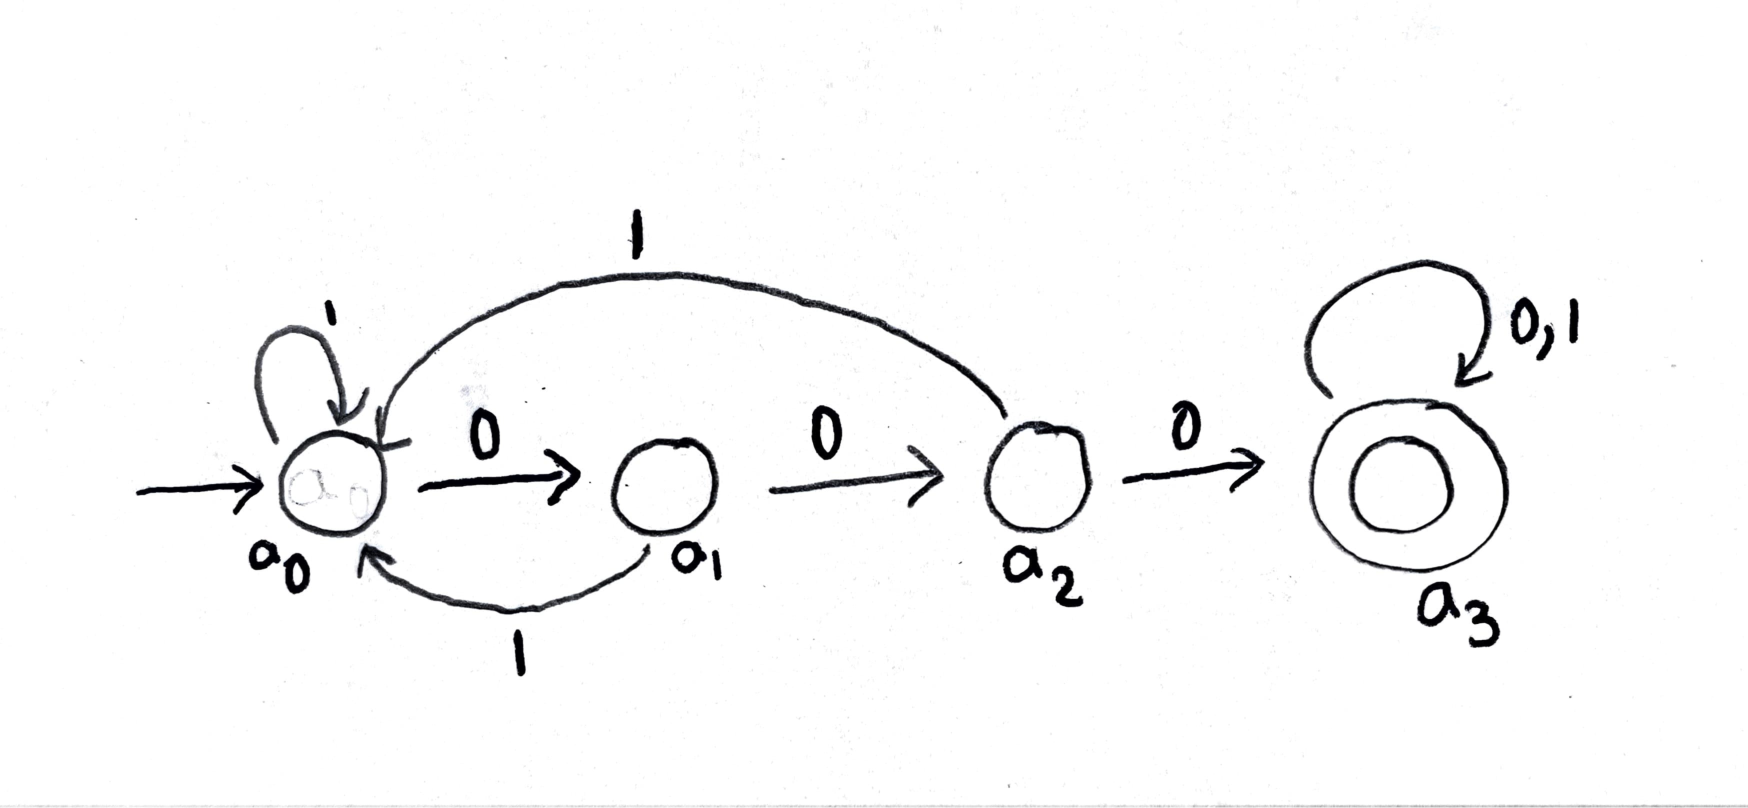
\includegraphics[width=10cm, height=5cm]{Week1b.pdf}
\end{center}
\indent c) The set of strings with 011 as a substring.
\medskip\begin{center}
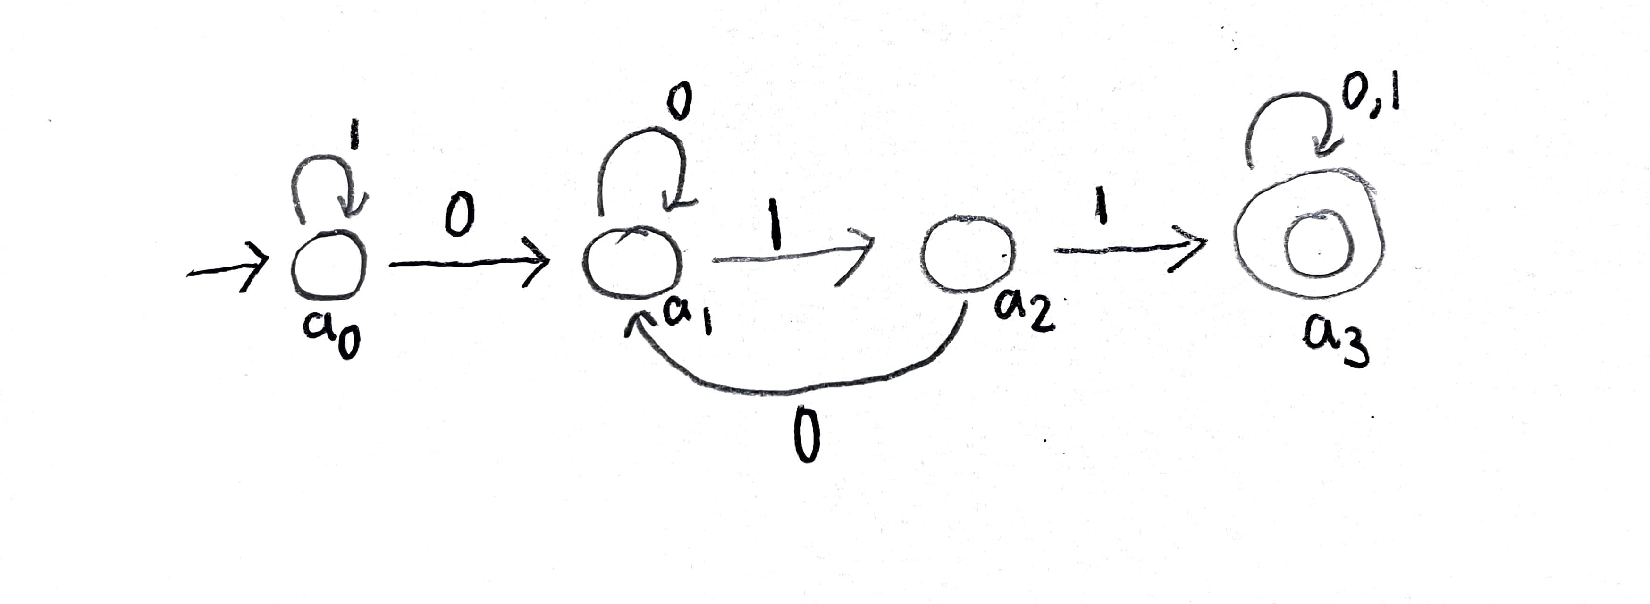
\includegraphics[width=10cm, height=5cm]{Week1c.pdf}
\end{center}

\subsection{Week 2: Regular Expression and NFA}
2.3.4: Give nondeterministic finite automata to accept the following languages. Try to take advantage of nondeterminism as much as possible. 
\medskip\begin{center}
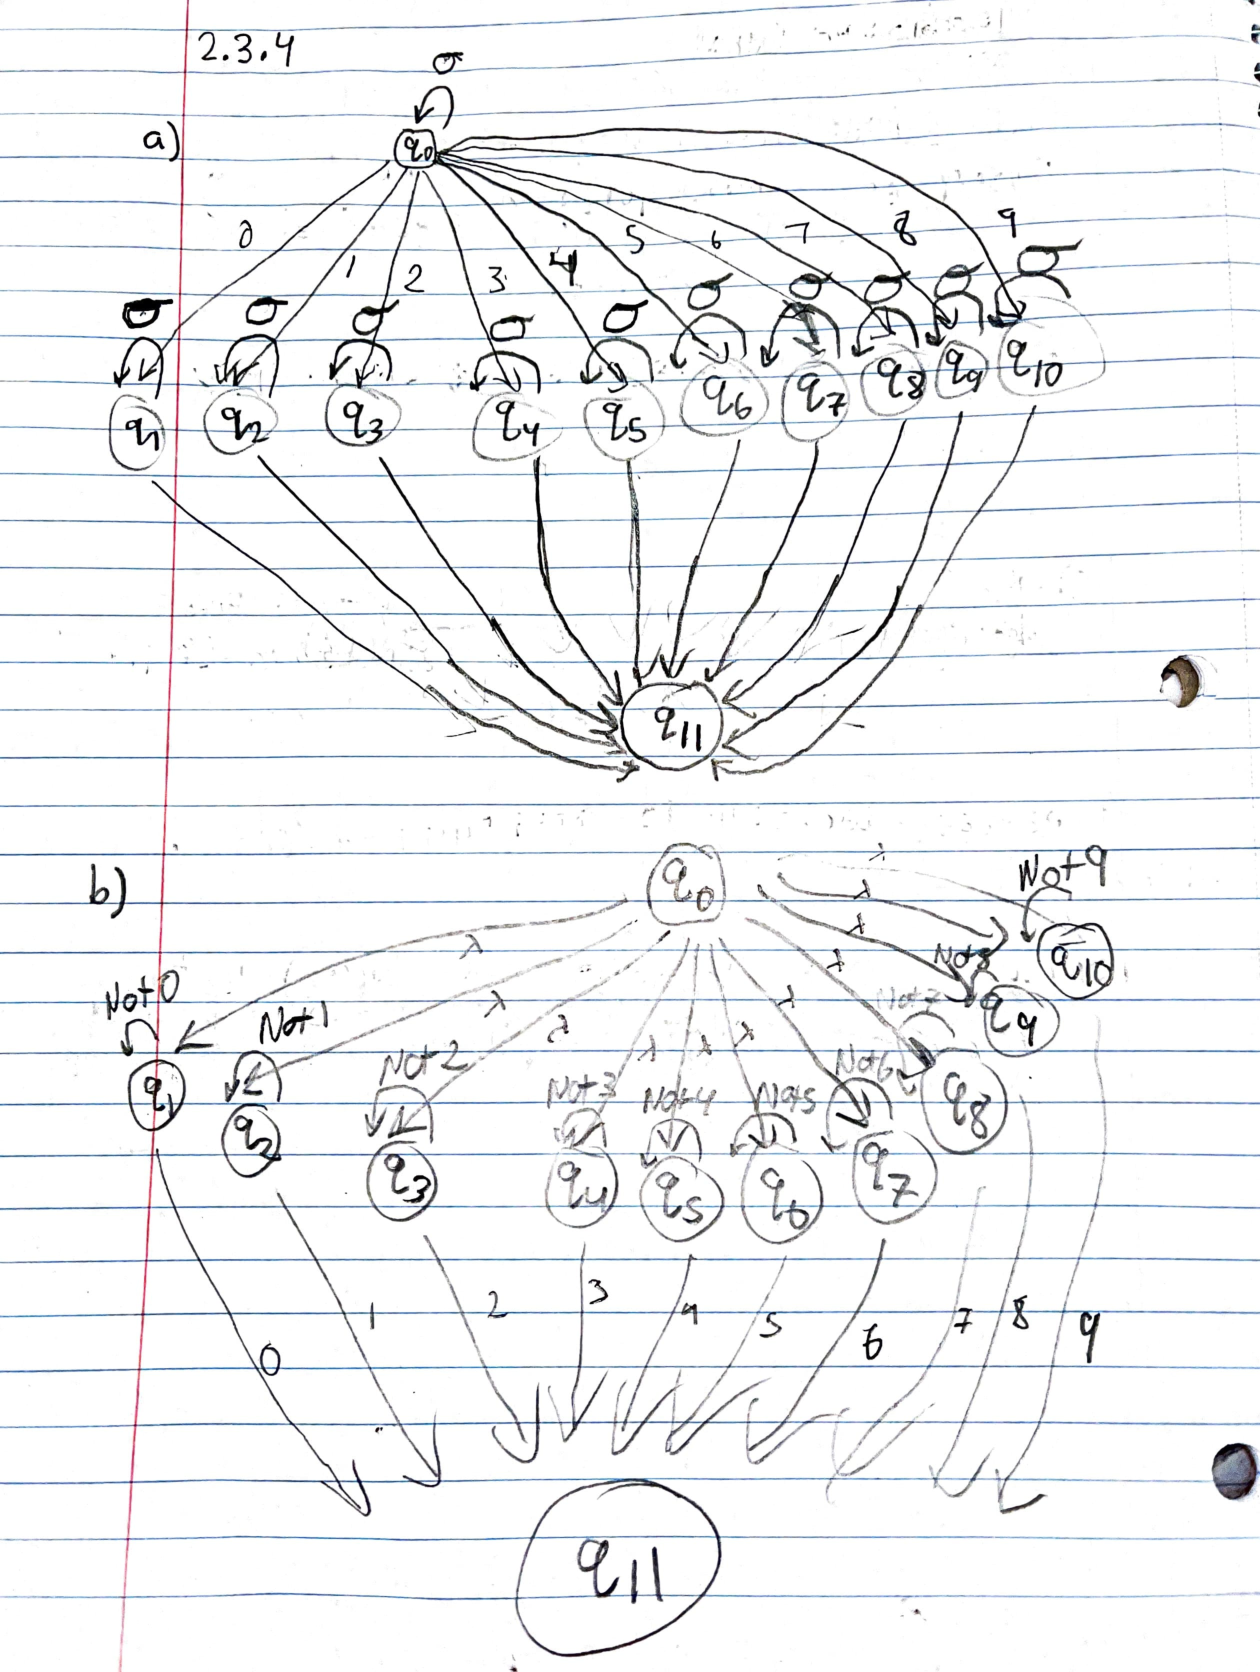
\includegraphics[width=10cm, height=15cm]{Week2_2.3.4ab.pdf}
\end{center}

\medskip\begin{center}
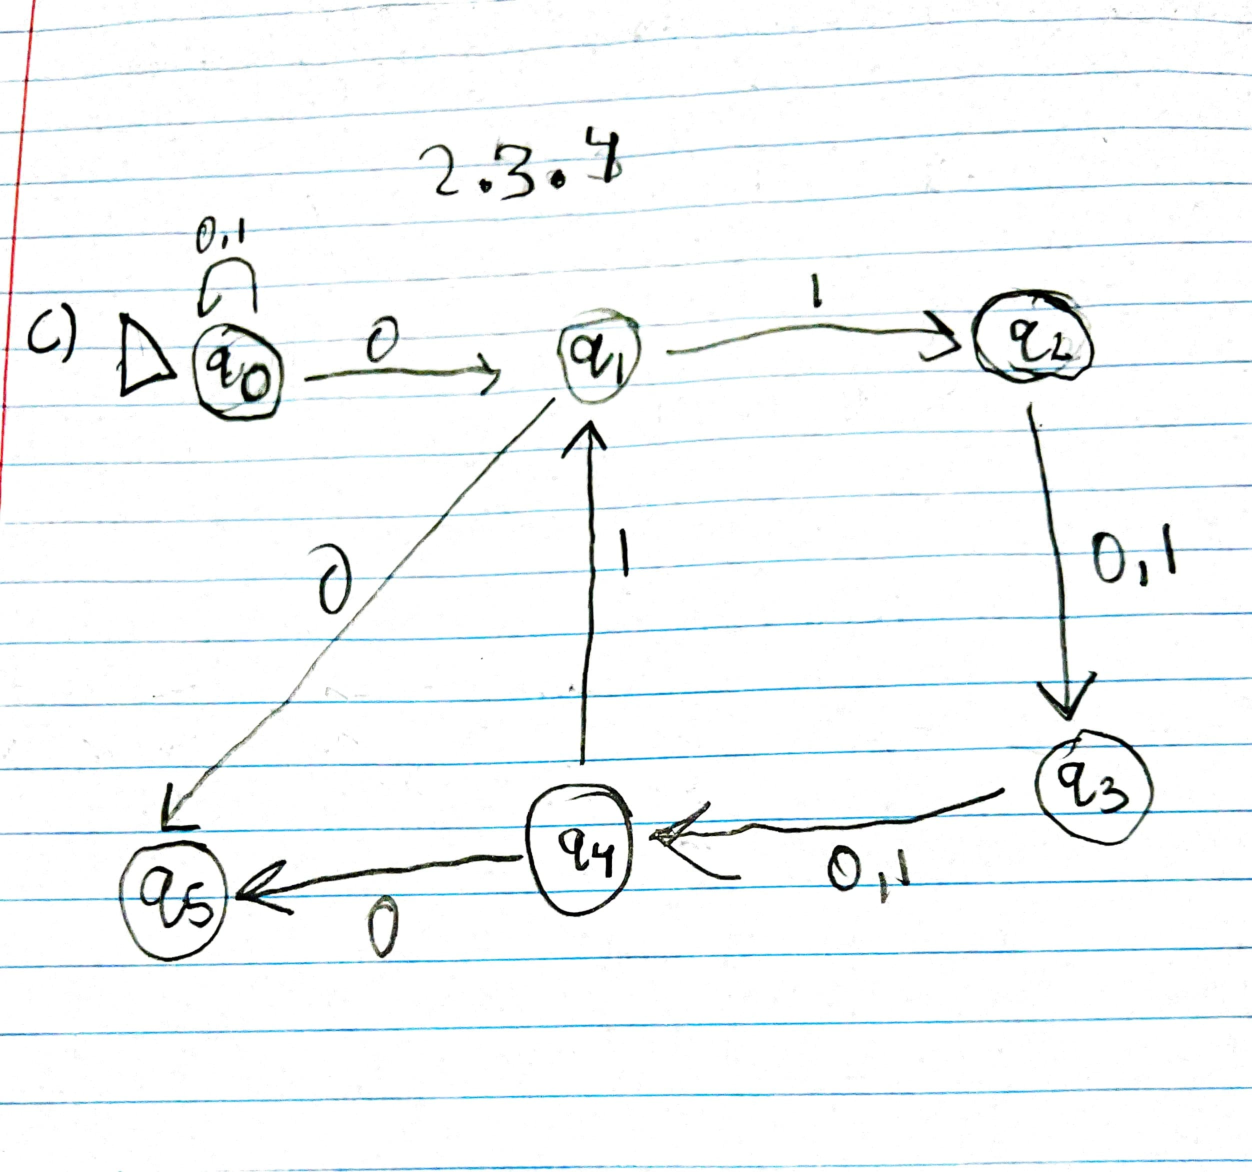
\includegraphics[width=10cm, height=10cm]{Week2_2.3.4c.pdf}
\end{center}

2.5.3: Design  $\epsilon$-NFA's for the following languages. Try to use $\epsilon$ transitions to simplify your design. 
\medskip\begin{center}
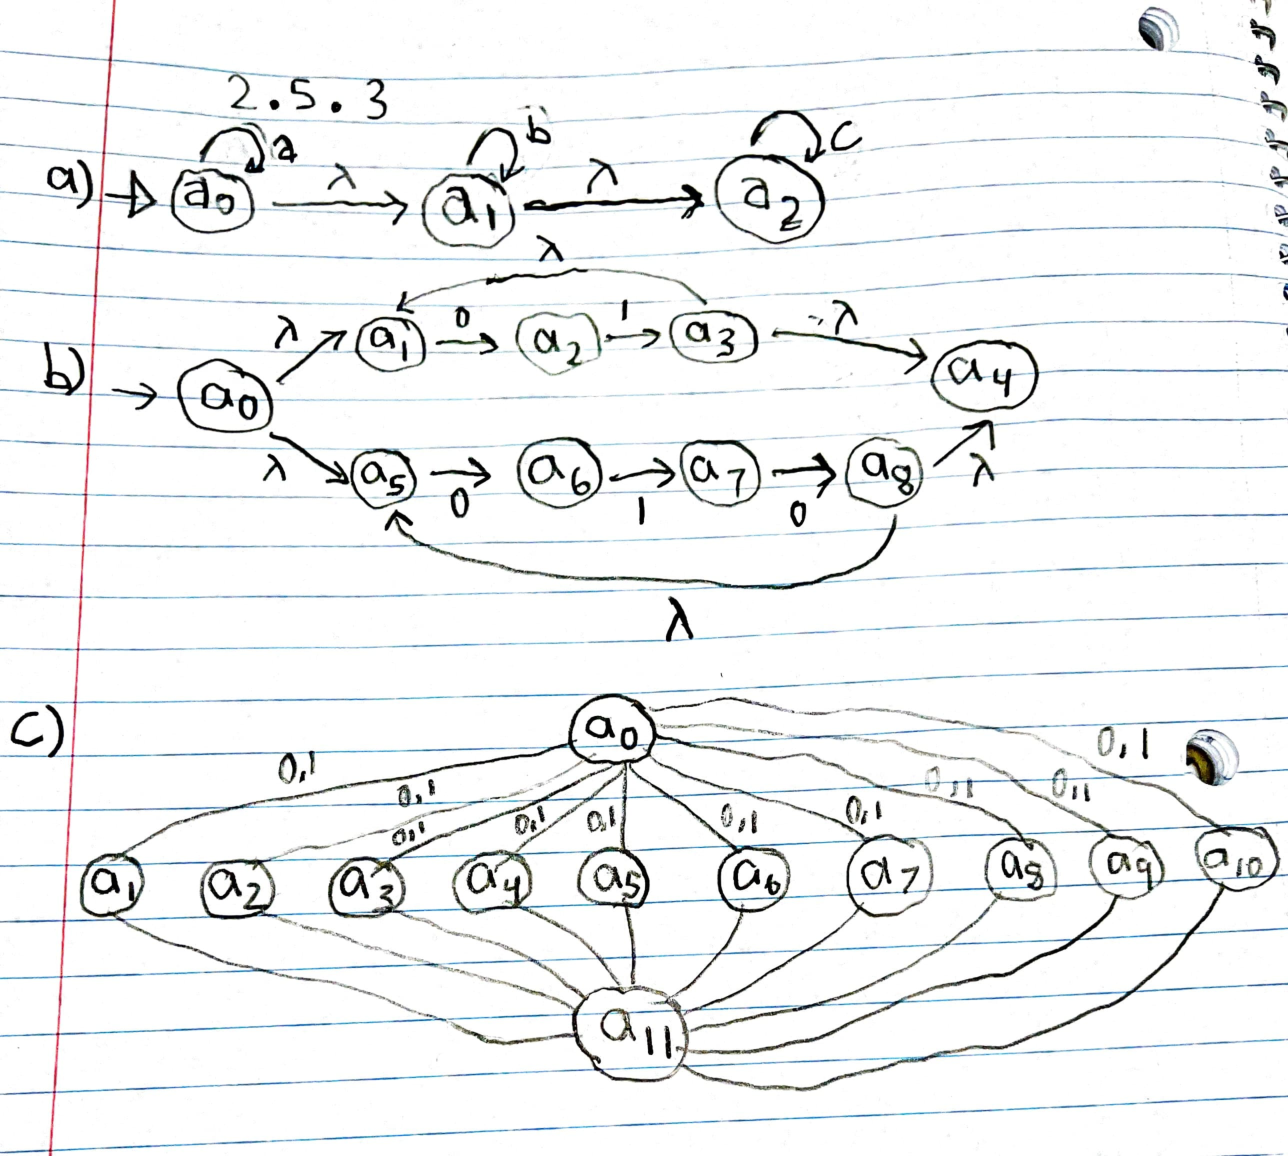
\includegraphics[width=10cm, height=10cm]{Week2_2.5.3.pdf}
\end{center}


\subsection{Week 3: Convert NFAs to DFAs by Hand}
2.3.1: Convert to a DFA the following NFA
\medskip\begin{center}
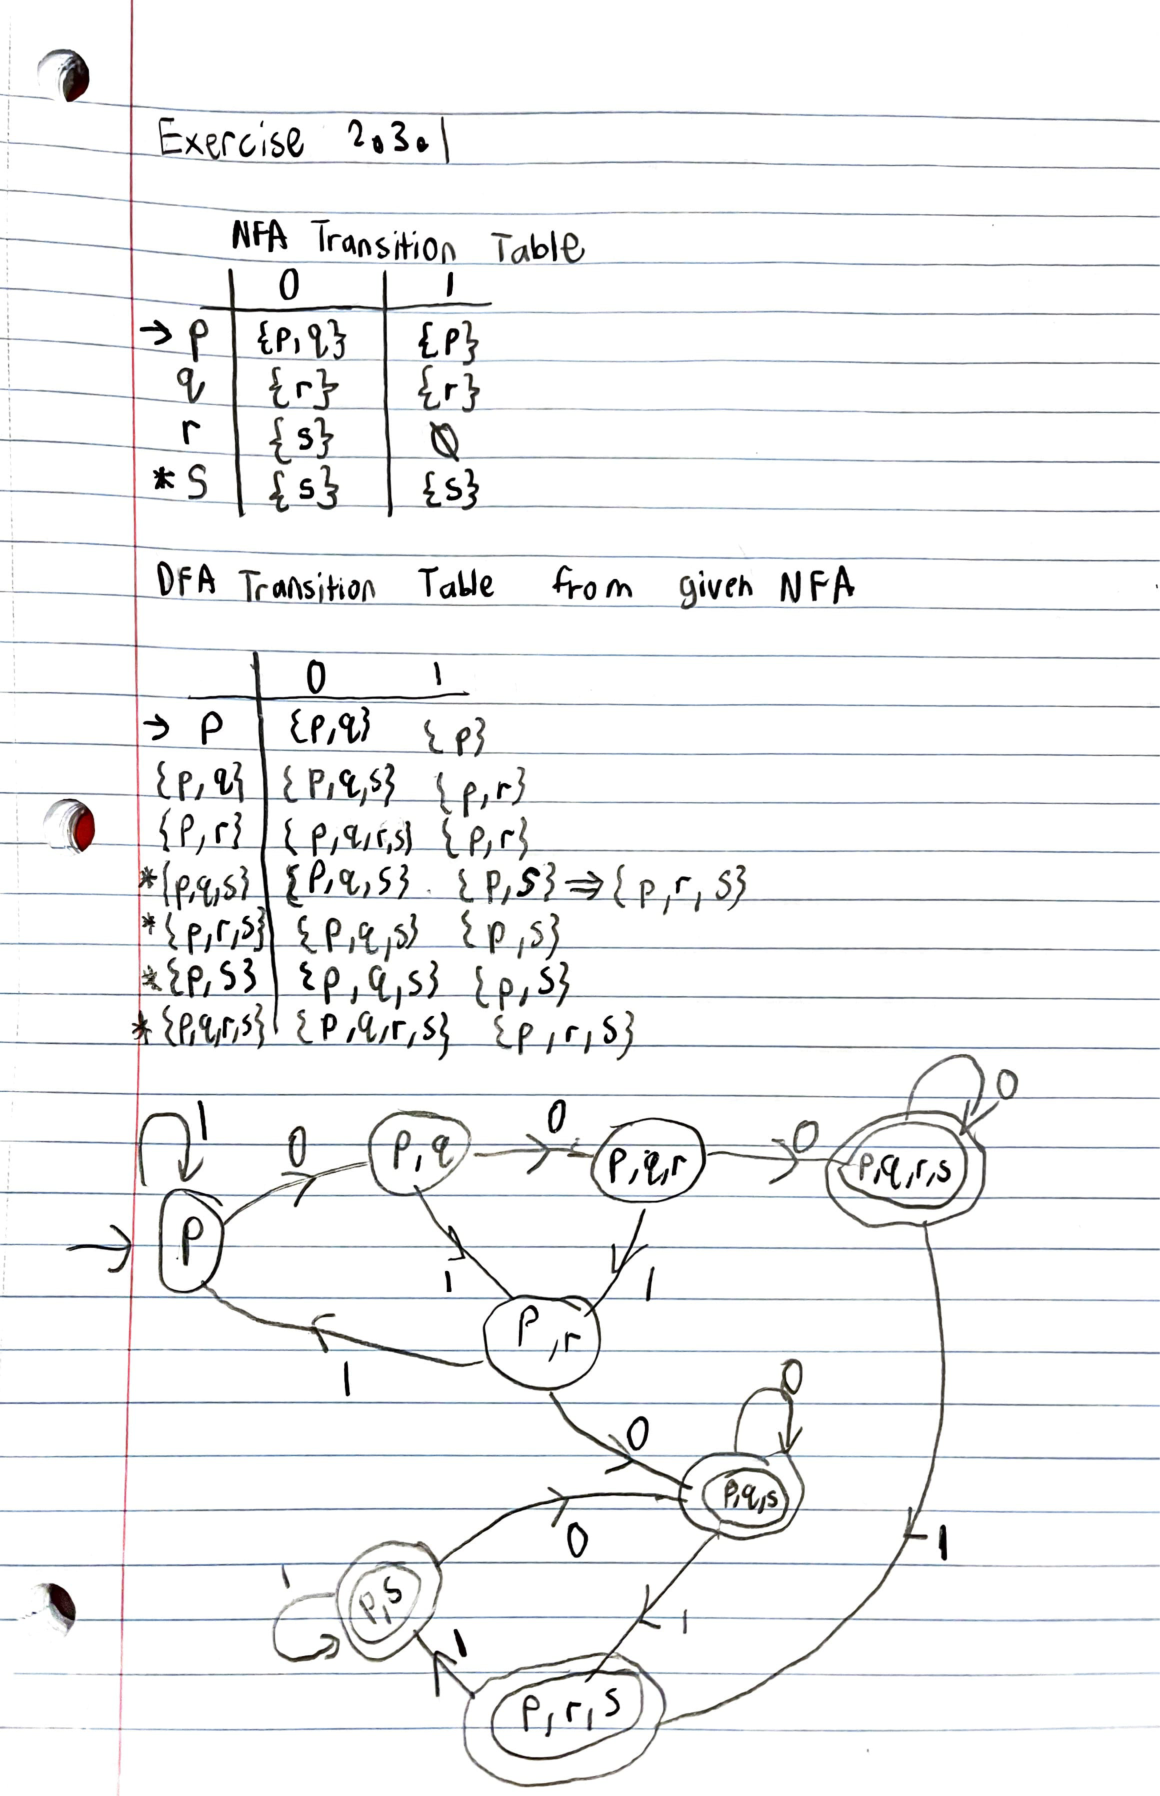
\includegraphics[width=10cm, height=15cm]{Week3_2.3.1.pdf}
\end{center}
2.3.2: Convert to a DFA the following NFA
\medskip\begin{center}
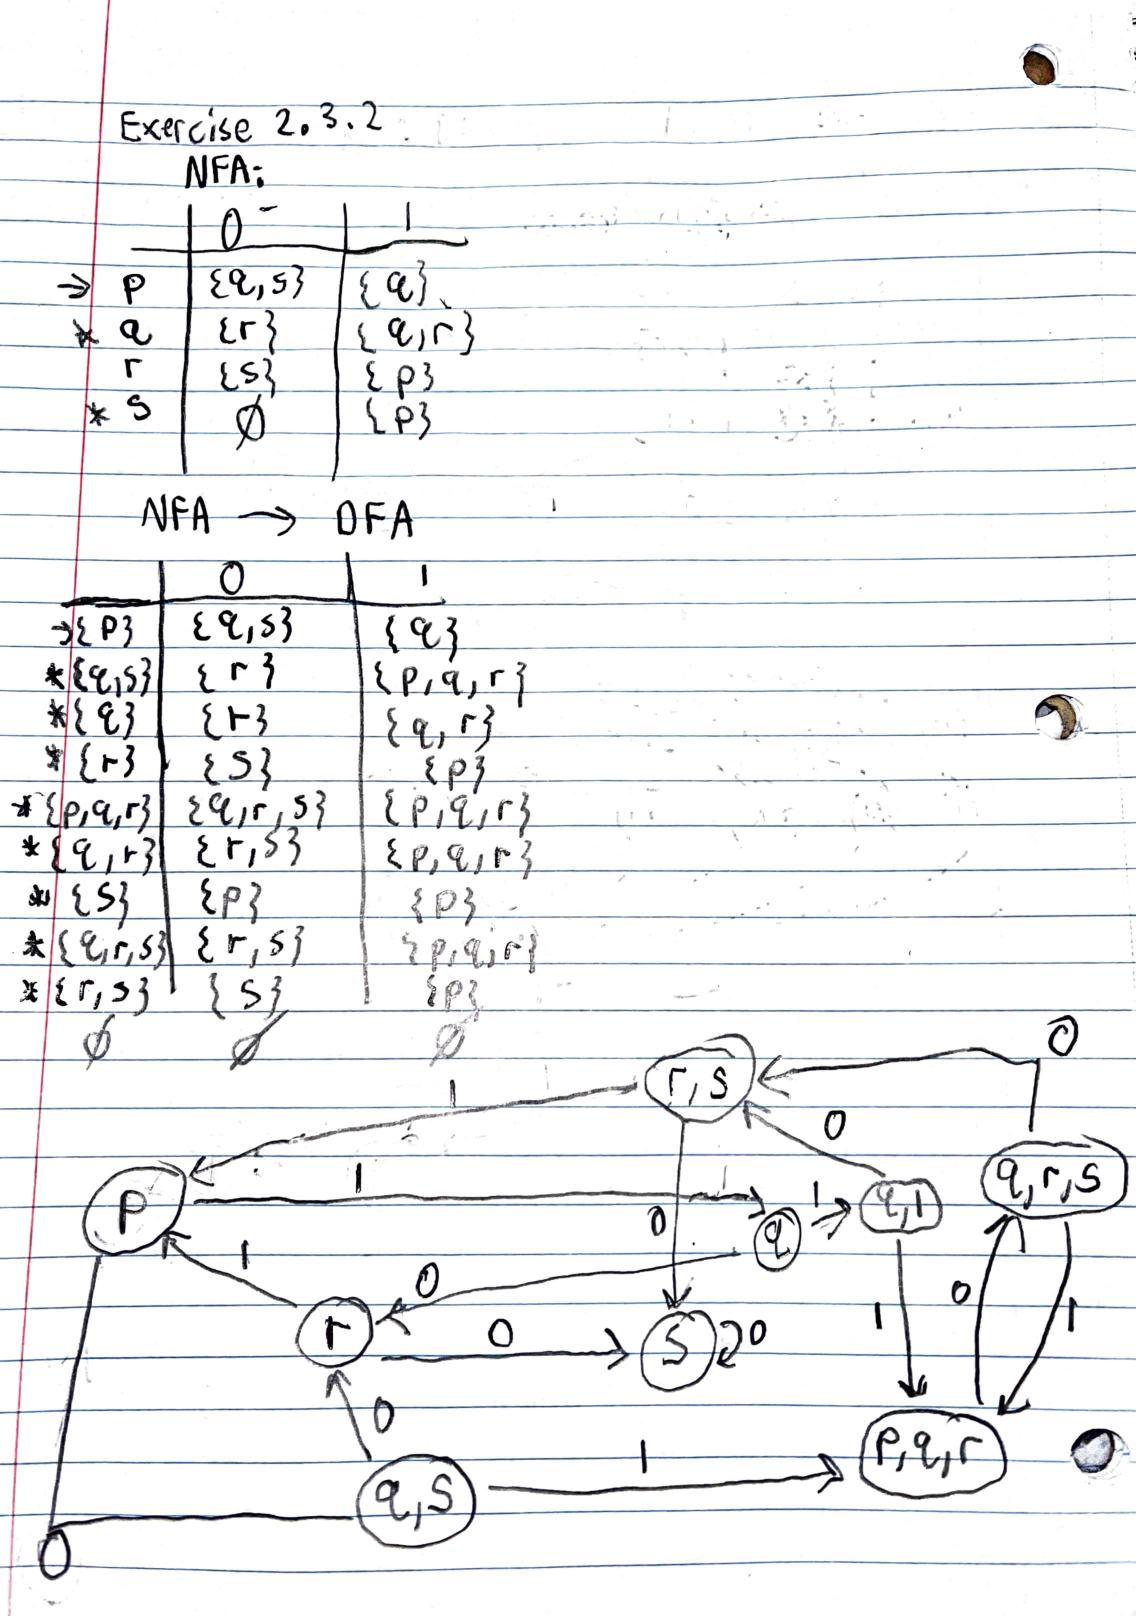
\includegraphics[width=10cm, height=15cm]{Week3_2.3.2.pdf}
\end{center}


\subsection{Week 4: Introduction to Parsing}
Question 1: Write out the parse tree (=concrete syntax tree) for the complete fibonacci program. Think about a question on this for the lecture.
\medskip\begin{center}
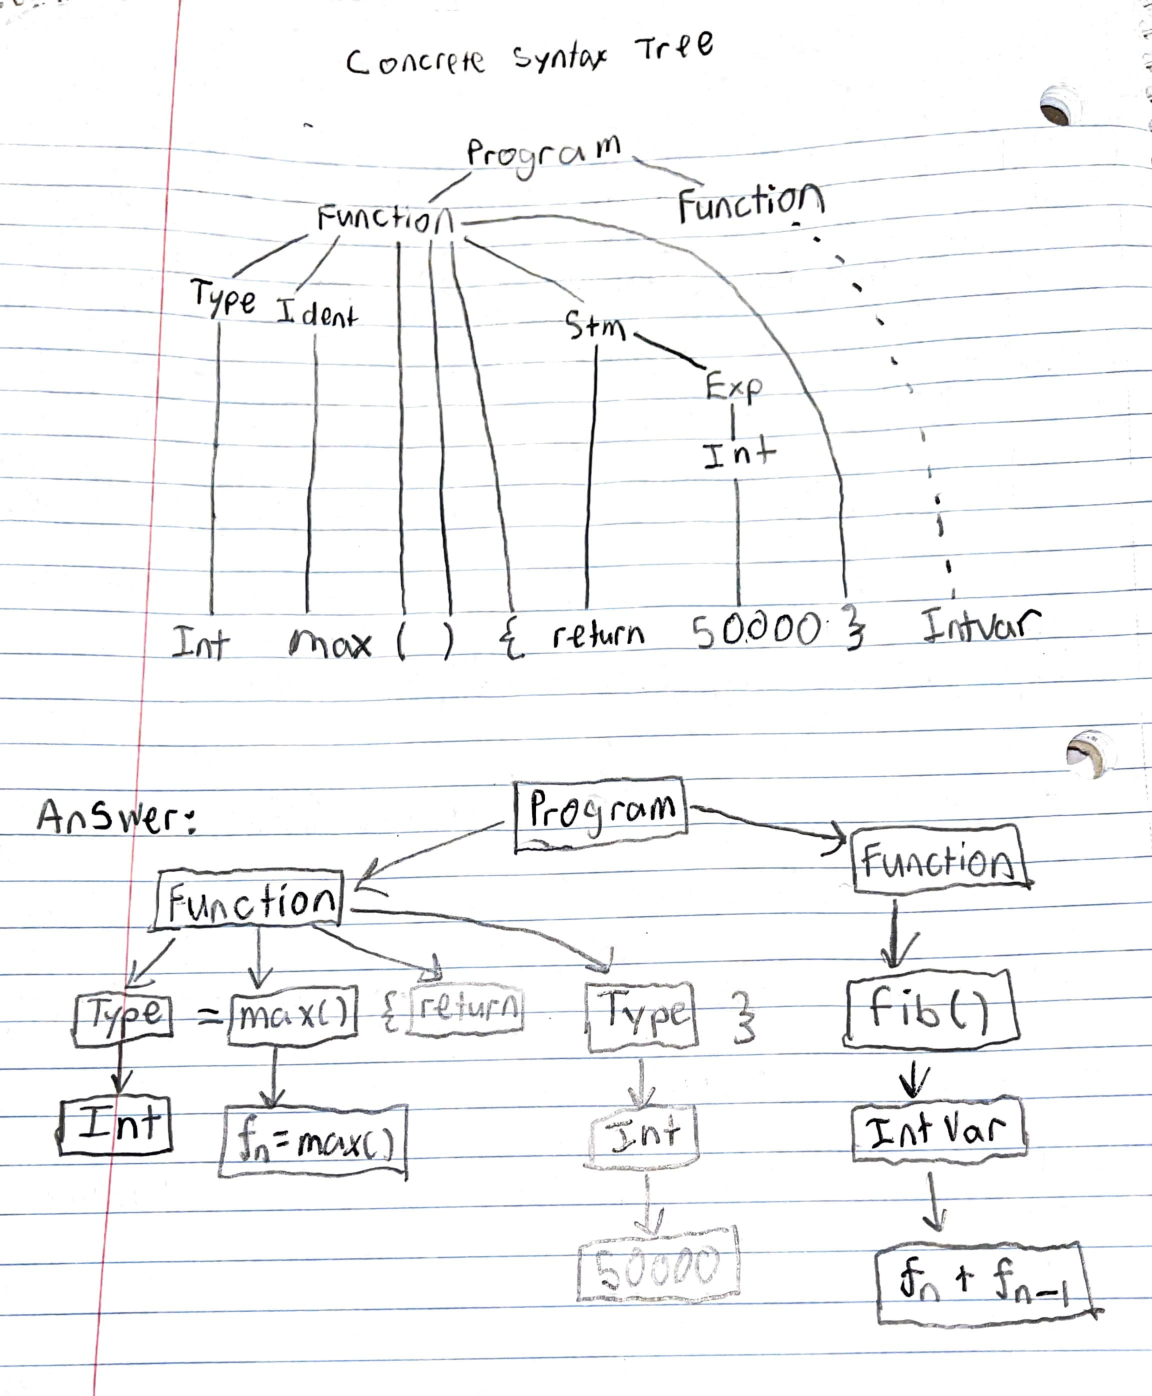
\includegraphics[width=10cm, height=15cm]{Week4Q1.pdf}
\end{center}
Question 2: Write out the abstract syntax tree for the complete fibonacci program. 
\medskip\begin{center}
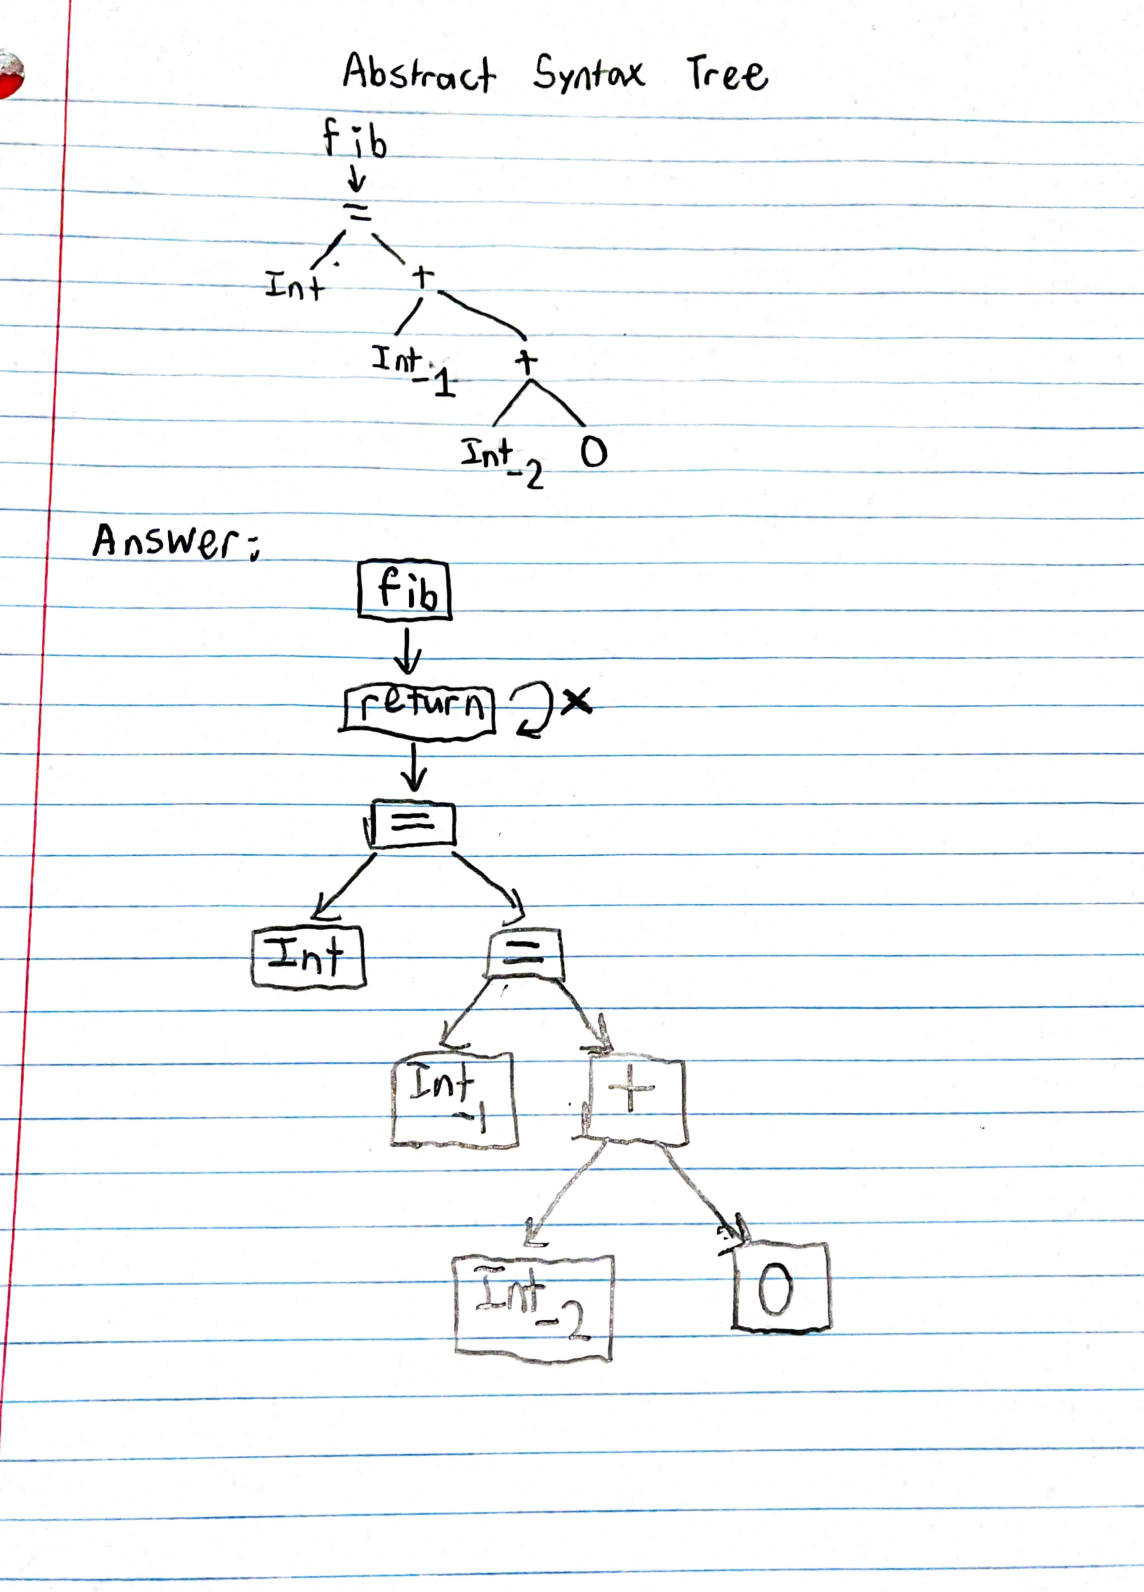
\includegraphics[width=10cm, height=15cm]{Week4Q2.pdf}
\end{center}

\subsection{Week 10: Proof Trees}
\medskip\begin{center}
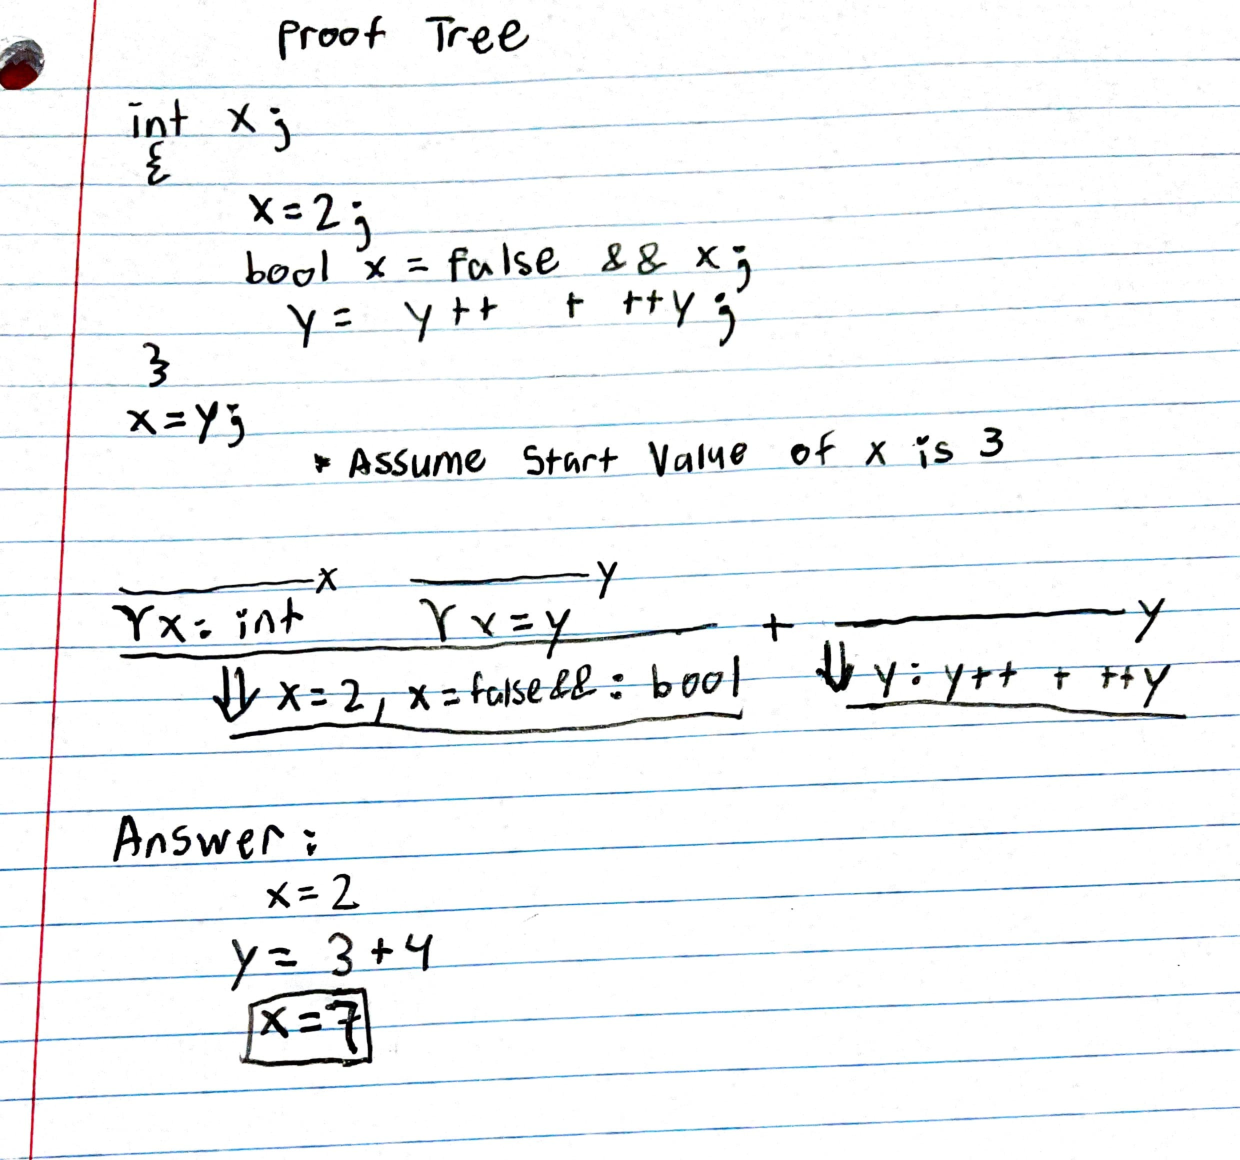
\includegraphics[width=10cm, height=15cm]{Week10.pdf}
\end{center}

\section{Project}
For this project, I plan to explain a compiler. The language that I would use is C++, and the compiler that I would use is g++. A code that I plan to use is a C++ code that convert Fahrenheit to Celsius, which is shown below. My target language would be JVM.
\begin{lstlisting}
#include <iostream>
double fahrenheitToCelsius(double fahrenheit){
    double celsius;
 
    celsius = (fahrenheit - 32.0) * 5.0 / 9.0;
    return celsius;
}
 
int main(){
    double fahrenheit;
 
    std::cout << "Enter temperature in fahrenheit (in degrees) ";
    std::cin  >> fahrenheit;
    std::cout << "Temperature in Celsius (in degrees) = "
              << fahrenheitToCelsius(fahrenheit) << std::endl;
}
\end{lstlisting}
Here is  output using x86-64 gcc 12.1
\begin{lstlisting}
fahrenheitToCelsius(double):
        push    rbp
        mov     rbp, rsp
        movsd   QWORD PTR [rbp-24], xmm0
        movsd   xmm0, QWORD PTR [rbp-24]
        movsd   xmm2, QWORD PTR .LC0[rip]
        movapd  xmm1, xmm0
        subsd   xmm1, xmm2
        movsd   xmm0, QWORD PTR .LC1[rip]
        mulsd   xmm0, xmm1
        movsd   xmm1, QWORD PTR .LC2[rip]
        divsd   xmm0, xmm1
        movsd   QWORD PTR [rbp-8], xmm0
        movsd   xmm0, QWORD PTR [rbp-8]
        movq    rax, xmm0
        movq    xmm0, rax
        pop     rbp
        ret
.LC3:
        .string "Enter temperature in fahrenheit (in degrees) "
.LC4:
        .string "Temperature in Celsius (in degrees) = "
main:
        push    rbp
        mov     rbp, rsp
        push    rbx
        sub     rsp, 24
        mov     esi, OFFSET FLAT:.LC3
        mov     edi, OFFSET FLAT:_ZSt4cout
        call    std::basic_ostream<char, std::char_traits<char> >& std::operator<< <std::char_traits<char> >(std::basic_ostream<char, std::char_traits<char> >&, char const*)
        lea     rax, [rbp-24]
        mov     rsi, rax
        mov     edi, OFFSET FLAT:_ZSt3cin
        call    std::basic_istream<char, std::char_traits<char> >::operator>>(double&)
        mov     esi, OFFSET FLAT:.LC4
        mov     edi, OFFSET FLAT:_ZSt4cout
        call    std::basic_ostream<char, std::char_traits<char> >& std::operator<< <std::char_traits<char> >(std::basic_ostream<char, std::char_traits<char> >&, char const*)
        mov     rbx, rax
        mov     rax, QWORD PTR [rbp-24]
        movq    xmm0, rax
        call    fahrenheitToCelsius(double)
        movq    rax, xmm0
        movq    xmm0, rax
        mov     rdi, rbx
        call    std::basic_ostream<char, std::char_traits<char> >::operator<<(double)
        mov     esi, OFFSET FLAT:_ZSt4endlIcSt11char_traitsIcEERSt13basic_ostreamIT_T0_ES6_
        mov     rdi, rax
        call    std::basic_ostream<char, std::char_traits<char> >::operator<<(std::basic_ostream<char, std::char_traits<char> >& (*)(std::basic_ostream<char, std::char_traits<char> >&))
        mov     eax, 0
        mov     rbx, QWORD PTR [rbp-8]
        leave
        ret
__static_initialization_and_destruction_0(int, int):
        push    rbp
        mov     rbp, rsp
        sub     rsp, 16
        mov     DWORD PTR [rbp-4], edi
        mov     DWORD PTR [rbp-8], esi
        cmp     DWORD PTR [rbp-4], 1
        jne     .L7
        cmp     DWORD PTR [rbp-8], 65535
        jne     .L7
        mov     edi, OFFSET FLAT:_ZStL8__ioinit
        call    std::ios_base::Init::Init() [complete object constructor]
        mov     edx, OFFSET FLAT:__dso_handle
        mov     esi, OFFSET FLAT:_ZStL8__ioinit
        mov     edi, OFFSET FLAT:_ZNSt8ios_base4InitD1Ev
        call    __cxa_atexit
.L7:
        nop
        leave
        ret
_GLOBAL__sub_I_fahrenheitToCelsius(double):
        push    rbp
        mov     rbp, rsp
        mov     esi, 65535
        mov     edi, 1
        call    __static_initialization_and_destruction_0(int, int)
        pop     rbp
        ret
.LC0:
        .long   0
        .long   1077936128
.LC1:
        .long   0
        .long   1075052544
.LC2:
        .long   0
        .long   1075970048
\end{lstlisting}


\subsection{Explaining Assembly Code for the FahrenheitToCelsius Function.}
Here is my code for fahrenheitToCelsius function:
\begin{lstlisting}
double fahrenheitToCelsius(double fahrenheit){
    double celsius;
 
    celsius = (fahrenheit - 32.0) * 5.0 / 9.0;
    return celsius;
}
\end{lstlisting}
 Here is fahrenheitToCelsius assembly code with line numbers:
\begin{lstlisting}
fahrenheitToCelsius(double):
        4 push    rbp
        5 mov     rbp, rsp
        6 movsd   QWORD PTR [rbp-24], xmm0
        7 movsd   xmm0, QWORD PTR [rbp-24]
        8 movsd   xmm2, QWORD PTR .LC0[rip]
        9 movapd  xmm1, xmm0
        10 subsd   xmm1, xmm2
        11 movsd   xmm0, QWORD PTR .LC1[rip]
        12 mulsd   xmm0, xmm1
        13 movsd   xmm1, QWORD PTR .LC2[rip]
        14 divsd   xmm0, xmm1
        15 movsd   QWORD PTR [rbp-8], xmm0
        16 movsd   xmm0, QWORD PTR [rbp-8]
        17 movq    rax, xmm0
        18 movq    xmm0, rax
        19 pop     rbp
        20 ret
\end{lstlisting}
Here is my explanation for the assembly code (the numbers correspond to each other).
\newline \newline 4. Save the old base pointer so that later the base pointer value can be restored for the caller when the function returns.
\newline \newline 5. Move the stack pointer into base pointer. This initial action maintains the base pointer to be used as a point of reference for finding parameters and local variables on the stack.
\newline \newline 6. Move the value of the register xmm0 which is the function parameter fahrenheit to a memory address at rbp(base pointe) with offset -24 bytes. 
\newline \newline 7. the value of parameter fahrenheit is stored into a floating point register xmm0.
\newline \newline 8. Move the value of memory address at LC0[rip], where rip pointer, which holds the value 32.0 to be stored into xmm2 register.
\newline \newline 9. moveapd refers to Move Aligned Packed Double Precision Floating - Point value, assign register xmm1 to hold the value of register xmm0. So xmm1 = xmm0 = value of fahrenheit. 
\newline \newline 10. Subtract the value of xmm1 with the value of xmm2, this corresponds to the code fahrenheit - 32.0.
\newline \newline 11. Move the value of memory address at LC1[rip] which holds 5.0 into xmm0 register. So xmm0 = 5.0.
\newline \newline 12. Multiply the value of xmm0 with xmm1, the result will be in xmm0. This correspond to the value of variable celsius being calculated as follows:
celcius = (fahrenehit - 32.0) * 5 
\newline \newline 13. Move the value 9.0 (from memory address at LC2[rip]) into xmm1.
\newline \newline 14. divide the value of xmm0 by the value of xmm1 
\newline \indent \indent xmm0 = celsius = (fahrenheit - 32.0) * 5.0
\newline \indent \indent xmm1 = 9.0
\newline This corresponds to the result of calculating: 
\newline \indent \indent celsius = ((fahrenheit - 32.0) * 5.0)/9.0
\newline  \indent xmm0 will have the value of variable celcius.
\newline \newline 15. The value of xmm0 (variable celsius) will be stored at memory address at rbp with offset - 8 bytes.
\newline \newline 16. Save the value of xmm0 (= varaible celsius).
\newline \newline 17. Move the value of xmm0 (= variable celsius) to rax register (general purpose register to hold function return value).
\newline \newline 18. Saved the function return value in xmm0 and rax register.
\newline \newline 19. Restore the caller's base pointer value by popping off (removing) rbp from the stack.
\newline \newline 20. Return to the caller and remove appropriate return address from the stack.

\subsection{Explaining Assembly Code for the Main Function.}
Here is my code for main function:
\begin{lstlisting}
18 int main()
19{
20    double fahrenheit; 
21
22    std::cout << "Enter temperature in fahrenheit (in degrees) ";
23    std::cin  >> fahrenheit;
24    std::cout << "Temperature in Celsius (in degrees) = "
25              << fahrenheitToCelsius(fahrenheit) << std::endl;
26 }
\end{lstlisting}
 Here is main function assembly code with line numbers:
\begin{lstlisting}
22 .LC3:
23         .string "Enter temperature in fahrenheit (in degrees) "
24 .LC4:
25         .string "Temperature in Celsius (in degrees) = "
26 main:
27 .LFB1746:
28         push    rbp
29         mov     rbp, rsp
30         push    rbx
31         sub     rsp, 24
32        mov     esi, OFFSET FLAT:.LC3
33        mov     edi, OFFSET FLAT:_ZSt4cout
34        call    _ZStlsISt11char_traitsIcEERSt13basic_ostreamIcT_ES5_PKc
35        lea     rax, [rbp-8]
36        mov     rsi, rax
37        mov     edi, OFFSET FLAT:_ZSt3cin
38        call    _ZNSirsERd
39        mov     esi, OFFSET FLAT:.LC4
40        mov     edi, OFFSET FLAT:_ZSt4cout
41        call    _ZStlsISt11char_traitsIcEERSt13basic_ostreamIcT_ES5_PKc
42	    mov     rbx, rax
43        mov     rax, QWORD PTR [rbp-24]
44        movq    xmm0, rax
45        call    _Z19fahrenheitToCelsiusd
46       movq    rax, xmm0
47        movq    xmm0, rax
48        mov     rdi, rbx
49        call    _ZNSolsEd
50        mov     esi, OFFSET FLAT:_ZSt4endlIcSt11char_traitsIcEERSt13basic_ostreamIT_T0_ES6_
51        mov     rdi, rax
52        call    _ZNSolsEPFRSoS_E
53        mov     eax, 0
54        mov     rbx, QWORD PTR [rbp-8]
55        leave
56        ret
\end{lstlisting}
Here is my explanation for the assembly code (the numbers correspond to each other).
\newline \newline 23. Assigned string value into register LC3.
\newline .LC3 will have string "Enter temperature in fahrenheit (in degrees)"
\newline \newline 25. Assigned string value into register LC4.
\newline .LC4 register will have "Temperature in Celsius (in degrees) ="
\newline \newline 28. save the old base pointer (rbp) value
\newline \newline 29. set the new base pointer (rbp) value to be the value of stack pointer (rsp)
\newline \newline 30. save the value of register rbx that the function will modify later. 
\newline \newline 31. make room for a 24 bytes local variable (fahrenheit);
\newline \newline 32. move the value of register LC3 into register esi.
\newline \newline 33. move the address of the standard library function cout into register edi.
\newline \newline 34. call standard library function cout. This code corresponds to C++ code line 22
\begin{lstlisting}
22    std::cout << "Enter temperature in fahrenheit (in degrees) ";
\end{lstlisting}
35. The value of address rbp-24 (base pointer with offset -24) is placed into register rax.
\newline \newline 36. Move the value of register ra into register rsi. 
\newline \newline 37. Move the address of the standard library function cin into register edi.
\newline \newline 38. Call standard library function cin. The value of register rax will be changed. Register rax will hold the value of the input variable fahrenheit. This code corresponds to C++ code on line 23.
\begin{lstlisting}
std::cin  >> fahrenheit;
\end{lstlisting}
39. Move the value of register LC4 into register esi. 
\newline \newline 40. Move the address of the standard library function cout into register edi.
\newline \newline 41. Call standard library function cout. This corresponds to C++ code line 24. 
\begin{lstlisting}
std::cout << "Temperature in Celsius (in degrees) = ";
\end{lstlisting}
42. Move the value of register rax(= variable fahrenheit) into register rbx.
\newline \newline 43. Move the value at address rbp-24 (rbp offset -24 byes) into rax register.
\newline \newline 44. Put the value of register rax into register xmm0. This assigns registers xmm0 to hold the value of variable fahrenheit. To calrify: rax = xmm0 = fahrenheit.
\newline \newline 45. Call the function fahrenheitToCelsius, this function will take xmm0 as parameter passed by the main function, which hold the input value of variable fahrenheit. This corresponds to C++ code line 25.
\begin{lstlisting}
<< fahrenheitToCelsius(fahrenheit) << std::endl;
\end{lstlisting}
46. Move the value of register xmm0 into register rax. xmm0 holds the return value from fahrenheitToCelsius function. Register xmm0 = register rax = new value of variable fahrenheit (which is the celsius value).
\newline \newline 47. Move register rax into register xmm0
\newline \newline 48. Move the value of register rbx into register rdi.
\newline \newline 49. Call the standard library cout function to display the new value of parameter fahrenheit returned by function fahrenheitToCelsius. Registers rax and xmm0 both hold the new value of fahrenheit, these registers will be accessed by the standard library cout function.
\newline \newline 50. Move the value specified by standard library endl (end of line) into register esi.
\newline \newline 51. Move the value of register rax into register rdi.
\newline \newline 52. Call the standard library function endl to put end of line in the output.
\newline \newline 53. Move 0 into register eax (initialize eax to 0)
\newline \newline 54. Move the value of the address at rbp(base stack) with offset - 8 bytes into register rbx, which will be used for transfer control.
\newline \newline 55. Leave the main function, pops the entire current stack and make registers available for other purposes.
\newline \newline 56. Return pops top of stack to the calling routine, in this case end of program execution.

\section{Conclusion}
This Compiler construction course materials along with the practical homeworks and assignments have thought me not only the idea of how a compiler work, but also how to design and implement a new language for a domain specific purpose. I find the flow of the materials from the beginning of the course to the end are very well phased and increasingly challenging.  For example, we learned how a simple mathematical expresion was parsed and translated into machine or binary language. I did not expect that by analyzing how compiler work in compiling my C++ program, I learned a better debbuggin skill and learned to write more efficient and better programs. Without the knowledge of how compiler and interpreter works, I think I might have a lot of frustration in debugging my prgram codes. After taking this course, I have  more confidence in software design and development and also design and implementation of a new programming language.  


\begin{thebibliography}{99}
\bibitem[HMU]{Hopcroft}
	John E. Hopcroft, Rajeev Motwani, Jeffrey D. Ullman:
\href{http://ce.sharif.edu/courses/94-95/1/ce414-2/resources/root/Text%20Books/Automata/John%20E.%20Hopcroft,%20Rajeev%20Motwani,%20Jeffrey%20D.%20Ullman-Introduction%20to%20Automata%20Theory,%20Languages,%20and%20Computations-Prentice%20Hall%20(2006).pdf}{Introduction to automata theory, languages, and computation,} 3rd Edition. Pearson international edition, Addison-Wesley 2007

\end{thebibliography}

\end{document}